\documentclass[tikz,border=12pt]{standalone}
% Shared visual language for standalone EMT block diagrams.
\usepackage{amsmath}
\usetikzlibrary{arrows.meta,backgrounds,calc,fit,positioning}

\tikzset{
    emt diagram/.style = {>={Stealth[length=2.4mm]}},
    line/.style        = {semithick, rounded corners=6pt},
    block/.style       = {draw, semithick, fill=white,
                          minimum height=1cm, minimum width=2.3cm},
    hblock/.style      = {block, minimum width=2.24cm, minimum height=1.3cm},
    vblock/.style      = {block, minimum width=1.3cm, minimum height=2.24cm},
    sum/.style         = {draw, semithick, fill=white, circle,
                          inner sep=2.6pt},
    signal/.style      = {circle, fill, inner sep=1.4pt,
                          label distance=3pt},
    sig/.style         = {font=\small},
    pm/.style          = {font=\scriptsize},
    wire jump/.style   = {line,
                          preaction={draw=white, line width=3pt,
                                     line cap=round}},
    enclosure/.style   = {draw, dashed, semithick, rounded corners=4pt},
    operator enclosure/.style = {enclosure, inner xsep=7mm, inner ysep=6mm}
}


\begin{document}
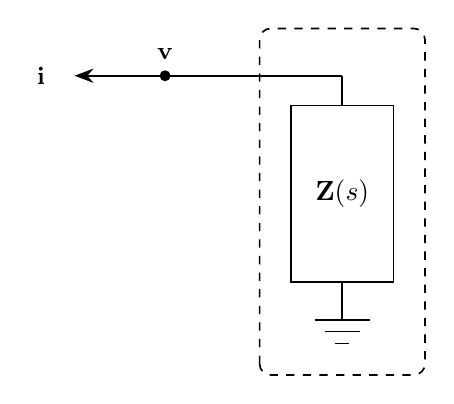
\begin{tikzpicture}[emt diagram]

% ================= Impedance branch =================
\node[vblock] (Z) at (0, -0.1) {$\mathbf{Z}(s)$};
\coordinate (terminal) at (0, 1.4);
\draw[line] (terminal) -- (Z.north);

% ================= Terminal voltage and current =================
\node[signal, label={[sig]above:$\mathbf{v}$}] (vport) at (-2.25, 1.4) {};
\draw[->, line] (terminal) -- (-3.4, 1.4);
\node[sig, anchor=east] at (-3.65, 1.4) {$\mathbf{i}$};

% ================= Ground reference =================
\draw[line] (Z.south) -- (0, -1.7);
\draw[semithick] (-0.35, -1.70) -- (0.35, -1.70);
\draw[semithick] (-0.22, -1.85) -- (0.22, -1.85);
\draw[semithick] (-0.09, -2.00) -- (0.09, -2.00);

% ================= Model enclosure =================
\draw[enclosure] (-1.05, -2.4) rectangle (1.05, 2.0);

\end{tikzpicture}
\end{document}
